\section{Methodology}
\label{sec:method}
In the subsequent sections, we describe the methodology which was used to conduct the literature review in more detail.

\subsection{Search Strategy}
Our literature review followed a systematic approach presented by Kitchenham~\cite{Kitchenham06}. The first step in our methodology was to search for existing literature reviews that focus on the same topic. Throughout the years several attempts have been made as seen in Chapter~\ref{sec:rel_work}. The most recent attempt we found is the work of Adilkhanov~\cite{Adilkhanov22}. However, their literature review focuses on devices used no matter the application. We in comparison want to focus on the entertainment industry specifically. Nevertheless, we used the taxonomy created by Adilkhanov as a first stepping stone to categorize the devices our literature review explored. We created a carefully crafted search term. The search term was designed to encompass the relevant literature to answer our research questions.

\begin{figure}[htbp]
	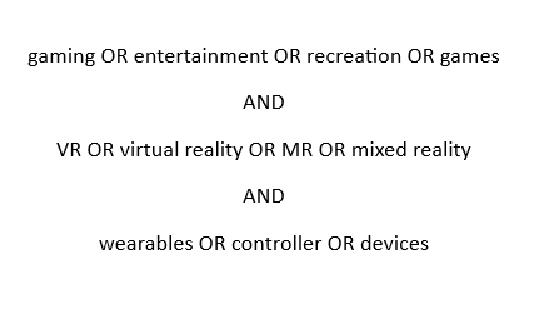
\includegraphics[width=\columnwidth]{figures/searchterm.pdf}
	\label{fig:searchterm}
	\caption{Search term, which was used to filter the IEEExplore Library}
\end{figure}


\subsection{Research Question}
We embarked on this research in the realm of entertainment because it is often challenging to obtain a comprehensive and timely overview of the latest developments in a certain sphere. Our aim is to provide a categorization guideline that enhances the clustering of future devices, making it easier for researchers and stakeholders in the industry to understand and navigate the landscape of MR and VR technologies. Additionally, we are interested in identifying the most frequently used devices within specific fields of application, shedding light on the devices that are driving innovation and adoption in the entertainment and gaming sector. 

\textbf{RQ1}~What are the developed devices in the last 5 years in Mixed Reality (MR) and Virtual Reality (VR), specifically focusing on entertainment? 

\textbf{RQ2}~What are the most common devices researched in the field of gaming and entertainment and how could they be categorized?

\subsection{Data Collection}
We conducted our literature search by querying the IEEEXplore library\footnote{https://ieeexplore.ieee.org/Xplore/home.jsp}, a well-known online database for computer science literature. This database was chosen due to its reputation and popularity among computer science studies. The initial search yielded a total of 699 results, representing potential sources for our review.

\subsection{Inclusion and Exclusion Criteria}
To narrow down our search results, we established a set of inclusion and exclusion criteria. These criteria were designed to ensure that the selected papers were both relevant and of high quality. Our inclusion criteria consisted of factors such as the publication date, the alignment with the research topic and, that a device was described in the study. On the other hand, the exclusion criteria were: papers were not written in English, were duplicate publications or had less than 4 pages.

\begin{description}
	\setlength\itemsep{-0.4em}
	\item[IC1] Studies must be relevant to VR or MR
	\item[IC2] Studies must discuss a device 
\end{description}

\begin{description}
	\setlength\itemsep{-0.4em}
	\item[EC1] Studies where full-text is not accessible
	\item[EC2] Studies that do not propose or extend a device
	\item[EC3] Studies that are not related to VR or MR
	\item[EC4] Studies not written in English
	\item[EC5] Proceedings where relevant study could not be identified
	\item[EC6] Studies with less than 4 pages
\end{description}


\subsection{Title Screening}
The next step involved a preliminary title screening of the 699 results. To distribute the workload efficiently, each member of our research team was assigned approximately one-third of the total results. After the title screening, 573 papers were excluded, as they did not meet our research objectives or failed to satisfy the inclusion criteria, leaving us with a reduced set of papers for further analysis.


\subsection{Full Paper Evaluation}
The remaining papers, totaling 126 articles, underwent a more thorough examination. During this phase, we manually filtered the content of each paper by reading the whole text. If a paper met all the inclusion criteria and did not meet any of the exclusion criteria, it was included. These assessments helped us identify the studies that would contribute devices to our literature review.

\subsection{Quality Assurance}
To ensure the validity of our review, we implemented a double-checking process. The papers that were included in our final selection was reviewed by another researcher of our team to confirm their suitability. Similarly, the papers that were excluded during the full paper evaluation were reviewed again by a different team member to reduce bias and the risk of excluding valuable contributions.

\subsection{Final Selection}
After our screening and quality assurance, a final set of 41 papers was identified as suitable for our literature review. These selected papers met our predefined inclusion criteria, demonstrated relevance to our research question by presenting a device related to VR or MR.

With this methodology, we provide a systematic and transparent approach to conducting our literature review.




%\begin{figure}[htbp]
%	\includegraphics[width=\columnwidth]{figures/definition_hierarchy.pdf}
%%	\label{fig:def_hierarchy}
%\end{figure}

